\subsection{Two-Stream Networks}
\begin{frame}{Separating Motion and Appearance}
    \begin{itemize}
        \item \textbf{Two-Stream Network:} Processes both RGB (appearance) and optical flow (motion) streams.
        \item Streams can be fused at various depths:
        \begin{itemize}
            \item \textit{Early fusion:} Combine features at initial layers.
            \item \textit{Late fusion:} Combine predictions or high-level features.
        \end{itemize}
        \item Improves robustness to background and enhances motion understanding.
    \end{itemize}
\end{frame}

\begin{frame}[allowframebreaks]{Two-Stream Network Architecture}
    \begin{figure}
        \centering
        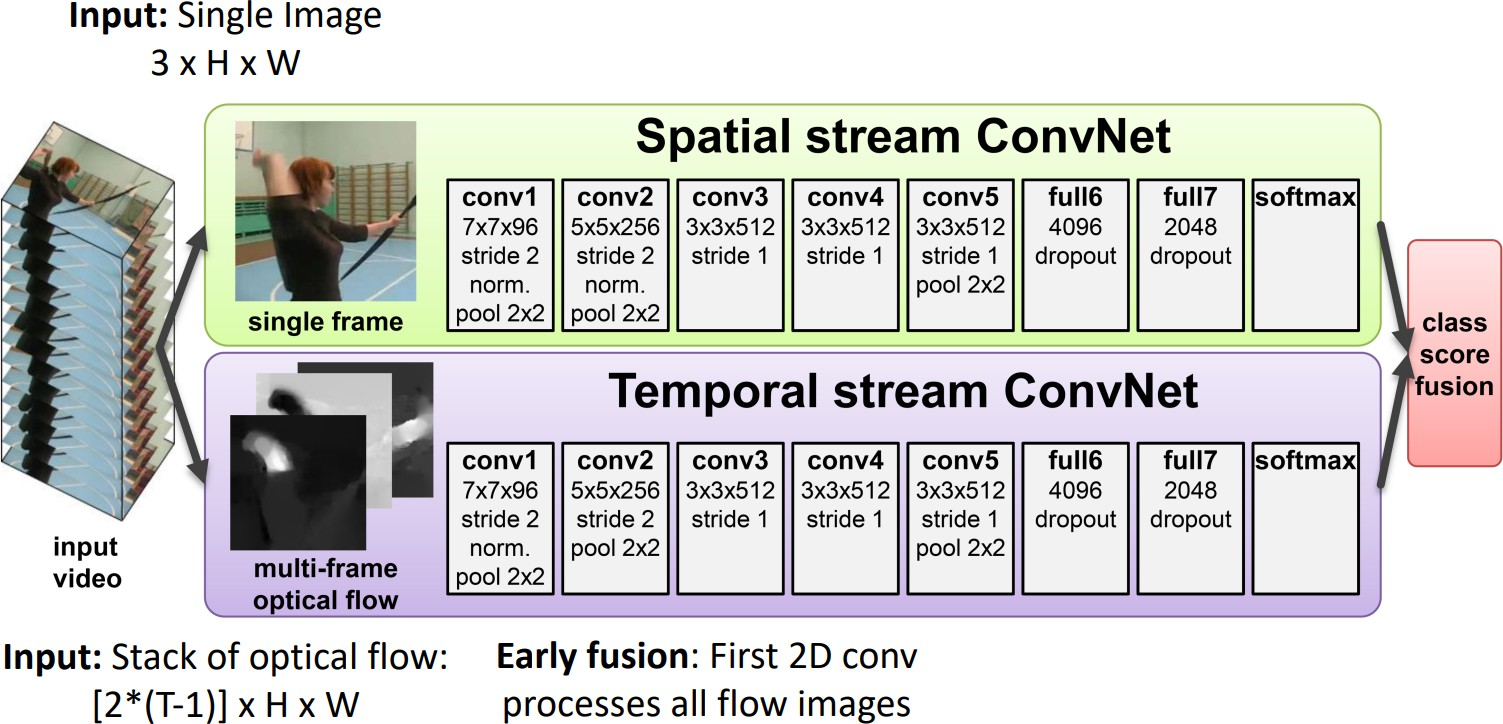
\includegraphics[width=1\textwidth,height=0.9\textheight,keepaspectratio]{images/video/slide_23_1_img.jpg}
    \end{figure}
\framebreak
    \begin{itemize}
        \item \textbf{RGB Stream:} Standard CNN (e.g., ResNet) for appearance features.
        \item \textbf{Optical Flow Stream:} Separate CNN for motion features.
        \item \textbf{Fusion:} Can be done at different stages:
        \begin{itemize}
            \item Early: Concatenate features from both streams.
            \item Late: Combine predictions from both streams.
        \end{itemize}
    \end{itemize}
\framebreak
    \begin{figure}
        \centering
        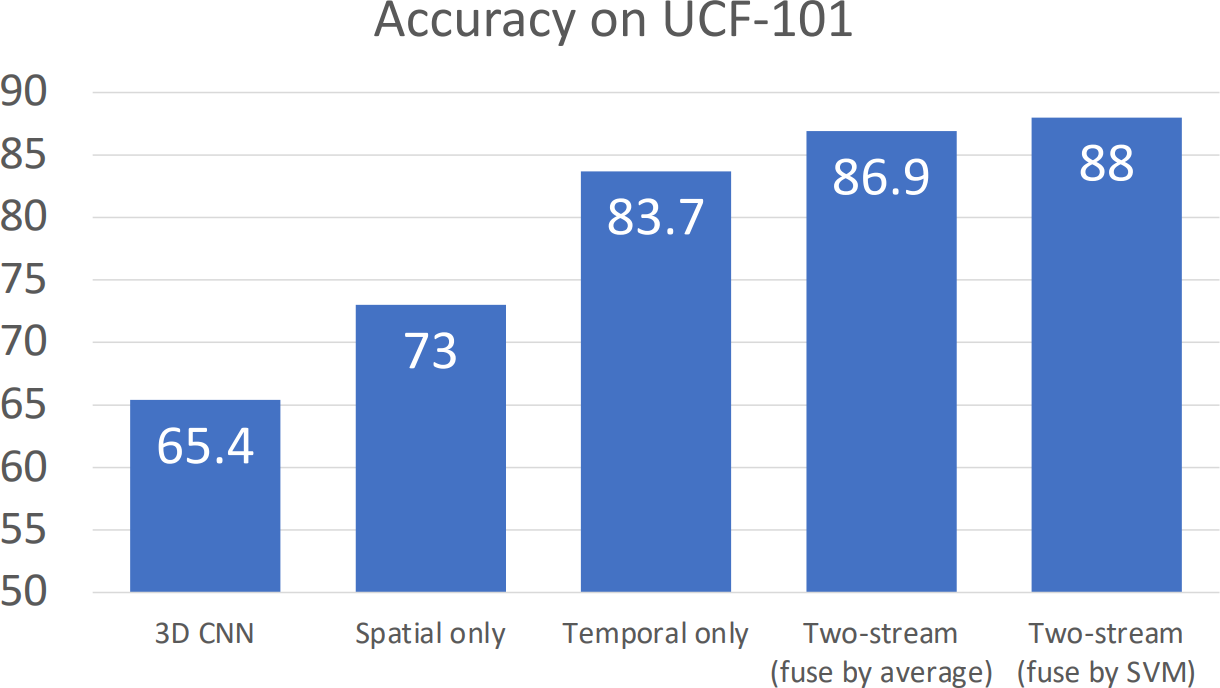
\includegraphics[width=1\textwidth,height=0.9\textheight,keepaspectratio]{images/video/slide_24_1_img.png}
    \end{figure}
\end{frame}